\capitulo{6}{Trabajos relacionados}

En este apartado voy a hablar sobre un proyecto parecido a este, pero que está actualmente funcionando. \\
La empresa Xiaomi tiene actualmente una aplicación como la mía en la tienda \textit{Google Play}, desde la cuál se pueden sincronizar los dispositivos Xiaomi que lo permitan y cambiar parámetros de ellos.

Actualmente, poseo una bombilla de esta marca como la de la imagen \ref{fig:yeelight} y cuenta con muchas posibilidades, entre ellas modificar su estado, color, intensidad y modo desde la propia aplicación de Xiaomi. Lo único que se necesita para que funcione es que el interruptor de la corriente esté encendido y que el dispositivo esté sincronizado con la aplicación.\\

\begin{figure}[h!]
	\centering
	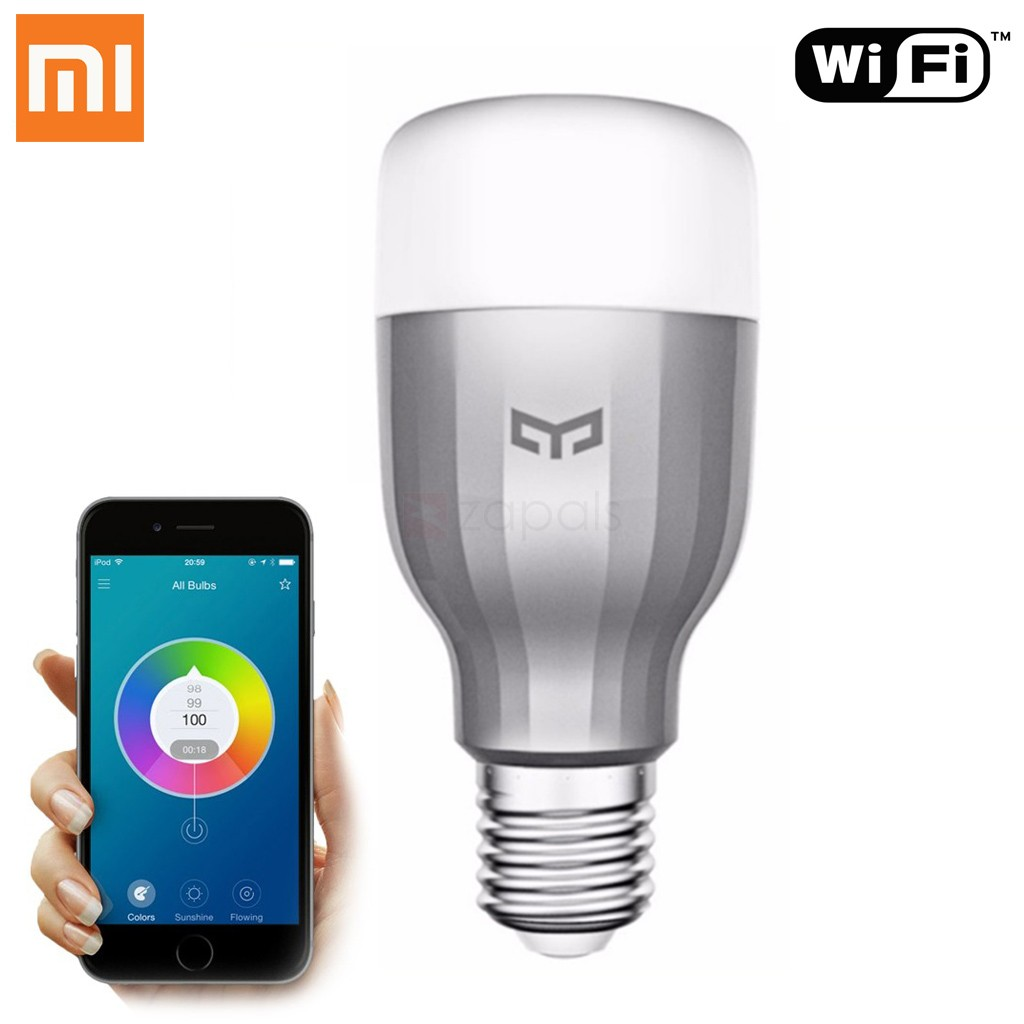
\includegraphics[width=0.35\linewidth]{img/xiaomiYeelight}
	\caption{Bombilla inteligente de la marca Xiaomi.}
	\label{fig:yeelight}
\end{figure}

La aplicación \textit{Mi Home} de Xiaomi se puede encontrar en \textit{Google Play} en el siguiente enlace \url{https://play.google.com/store/apps/details?id=com.xiaomi.smarthome&hl=es}.